\section[Limits on $t\bar{t}t\bar{t}$ production]{Limits on \boldmath{$t\bar{t}t\bar{t}$} production}

As discussed previously, the 1-lepton search is also used to set limits on four-top-quark production considering different signal benchmark scenarios: SM $t\bar{t}t\bar{t}$ production, $t\bar{t}t\bar{t}$ production via an EFT model with a four-top contact interaction, and $t\bar{t}t\bar{t}$ production in a Universal Extra Dimension (UED) model with two extra dimensions compactified under the Real Projective Plane (RPP) geometry.\par
In the case of $t\bar{t}t\bar{t}$ production within the SM, the observed (expected) $95\%$ CL upper limit on the production cross section is 130 fb (110 fb), or 15 (12) times the SM prediction.
In this scenario the expected sensitivity of this analysis is improved compared to that of previous ATLAS searches \cite{ATLAS-CONF-2016-013,ATLAS-CONF-2016-020}. The CMS Collaboration has performed as well a search in this scenario reporting an observed (expected) $95\%$ CL upper limit on the production cross section of 10.2 (10.8) times the SM prediction \cite{CMS-PAS-TOP-16-016}.\par
In the case of $t\bar{t}t\bar{t}$  production via an EFT model with a four-top contact interaction, the observed (expected) $95\%$ CL upper limit on the production cross section is 51 fb (54 fb). The improved sensitivity in the case of the EFT model results from the harder $m_{\rm eff}$ spectrum compared to that of SM $t\bar{t}t\bar{t}$ production. The upper limit on the production cross section can be translated into an observed (expected) limit on the free parameter of the model: $|C_{4t}|/\Lambda^{2} < 2.9$ $\tev^{-2}$ ($3.0$ \tev$^{-2}$).\\ \indent
Finally, the observed and expected upper limits on the production cross section times branching ratio for the UED model are shown in figure \ref{sec:vlq:fig:uedrpp} as a function of $m_{KK}$ for the symmetric case ($\xi = R_{4}/R_{5} = 1$), assuming production by tier (1,1) alone. The comparison to the LO theoretical cross section sets an observed (expected) $95\%$ CL lower limit on $m_{KK}$ of 1.6 $\tev$ (1.5 \tev). \\ \indent
In summary, the search presented here obtains the most restrictive limits to date for BSM $t\bar{t}t\bar{t}$ production in the various new physics scenarios considered.


\begin{figure}[t!]
 \centering
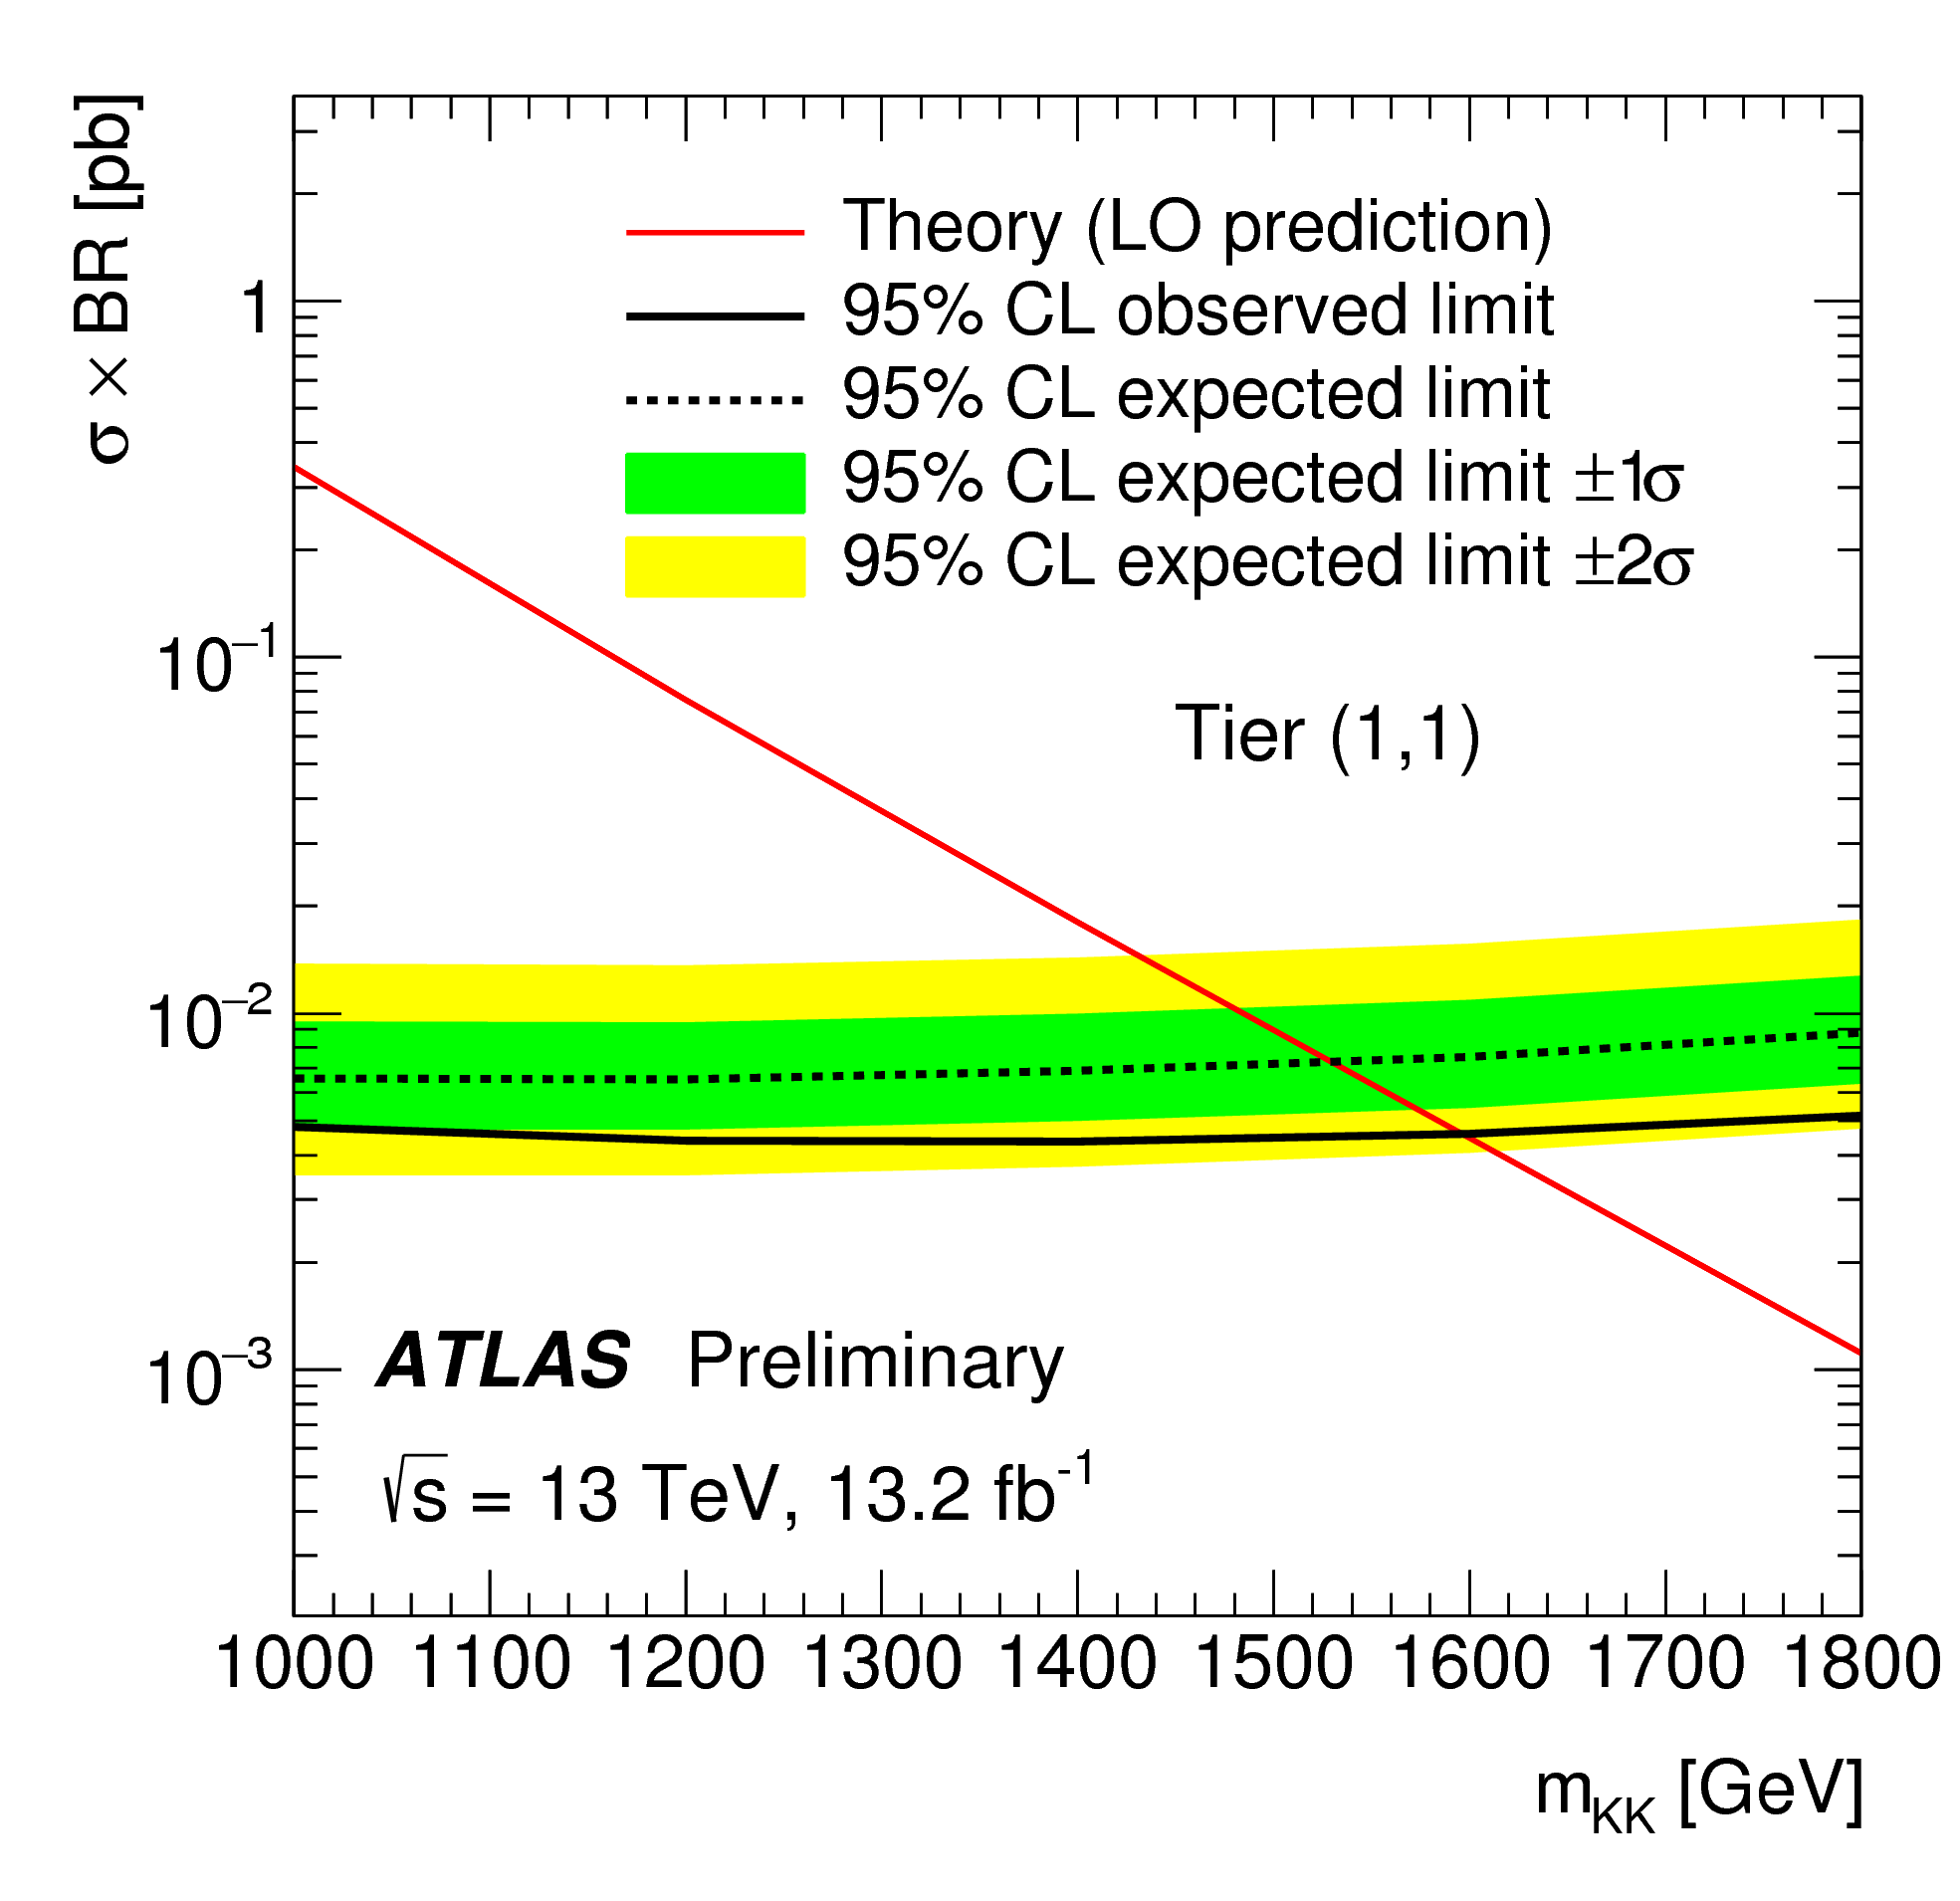
\includegraphics[width=0.5\textwidth]{figures/VLQ/fig_20.png}
\captionsetup{width=0.85\textwidth} \caption{\small Observed (solid line) and expected (dashed line) 95\% CL upper limits on the production cross section times branching ratio
of four-top-quark events as a function of the Kaluza--Klein mass ($m_{KK}$) from tier (1,1) in the symmetric case ($\xi=R_4/R_5=1$).
The surrounding shaded bands correspond to $\pm1$ and $\pm2$ standard deviations around the expected limit. 
The thin red line shows the theoretical prediction, computed at LO in QCD, for the production cross section of four-top-quark events 
by tier (1,1) assuming $BR(A^{(1,1)}\to t\bar{t})=1$, where the heavy photon $A^{(1,1)}$ is the lightest particle of this tier.}
\label{sec:vlq:fig:uedrpp}
\end{figure}
